\documentclass[12pt]{article}
%% \usepackage{bookman}
\usepackage{hyperref}
\usepackage{graphicx}
\usepackage{sidecap}
\usepackage[numbers]{natbib} 
\usepackage[font=small,labelfont=sf, margin=1in]{caption}
\usepackage{rotating}

\hypersetup{
  % bookmarks=true,         % show bookmarks bar?
    unicode=false,          % non-Latin characters in Acrobat’s bookmarks
    pdftoolbar=true,        % show Acrobat’s toolbar?
    pdfmenubar=true,        % show Acrobat’s menu?
    pdffitwindow=false,     % window fit to page when opened
    pdfstartview={FitH},    % fits the width of the page to the window
    pdftitle={Thesis Proposal},
    pdfauthor={Wei Liu},     % author
    pdfsubject={Wei Liu's Thesis Proposal},   % subject of the document
    pdfcreator={Wei Liu},   % creator of the document
    pdfproducer={Wei Liu}, % producer of the document
    pdfkeywords={Thesis Proposal, fmri, functional brain connectivity}, % list of keywords
    pdfnewwindow=true,      % links in new window
    colorlinks= true,       % false: boxed links; true: colored links
    linkcolor=blue,          % color of internal links
    citecolor=blue,        % color of links to bibliography
    filecolor=magenta,      % color of file links
    urlcolor=cyan           % color of external links
}

\setlength{\oddsidemargin}{0 in}
\setlength{\evensidemargin}{0 in}
\setlength{\topmargin}{-1 in}
\setlength{\textwidth}{6.5 in}
\setlength{\textheight}{9 in}
\setlength{\headsep}{0.5 in}
\setlength{\parindent}{0 in}
\setlength{\parskip}{0.1 in}

\begin{document}
\title{Thesis Proposal}
\author{Wei Liu\\ \small{(advisor: Tom Fletcher)} }
\date{\today} 

\maketitle 
\begin{center}
\noindent{Committee:}\\
Jeff Anderson \\
Suyash Awate \\
Tom Fletcher\\
Guido Gerig\\
Tolga Tasdizen
\end{center}

%% \abstract{Resting-state fMRI is widely used to study the mapping of brain's
%%   functional network. Such study typically starts by defining a set of
%%   nodes and then estimate the functional connections between them. For group
%%   study, a summary network map is usually estimated from individual's map. In
%%   this proposal, I aim to estimate the functional connectivity with clustering
%%   based methods with each voxel defined as a variable. We also take context
%%   information into account. \emph{Context} here means 1) the spatial neighbors of
%%   variables at each voxel in order to get spatially coherence network maps, and
%%   2) the variables at same spatial location of other subjects and population
%%   network map, in order to build a multi-level network map including group and
%%   subject levels. The group functional map estimated from such model respects the
%%   variablity among subjects, as well as collecting all shared information of them.
 
%% }

%% \textbf{Alternative Abstract:} In brain connectivity study using resting-state
%% functional MRI images, a summary of the group of subjects is estimated typically
%% by simple averaging the individual's functional networks. I propose a
%% hierarchical model that explicitly represent the relationship of the group and
%% the subjects functional network using Markov Random Field (MRF).  The novelty of
%% our method is both group and each subject's network are obtained simultaneously
%% in a unified clustering-based algorithm, and subject network maps use group as a
%% prior. Furthermore, the spatial context information is modeled by MRF instead of
%% being enforced by the conventional spatial smoothing in preprocessing steps. I
%% will show the modeling of group and spatial neighbor's network information
%% improves identifying subject's network, and hence also helps obtaining a
%% consistent group network map.}

\section{Introduction}

\section{Problem Statement}
%% The goal of my research is to characterize the functional connectivity among the
%% regions or voxels of the human brain cortex by using resting-state fMRI. I build
%% hierarchical models and computational methods and verify that the hierarchical
%% model can identify consistent connectivity among multiple subjects, while repecting
%% each subjects variability.

\begin{center}
\parbox{5in}{\emph{The goal of my research is to identify the functional
    connectivity of the human brain cortex by using resting-state fMRI. I build
    hierarchical models for consistent estimation of both population and
    individual subject's functional network map, and use Markov Random Field to
    represent the context information within and across subjects.}}
\end{center}

Alternative:

\begin{center}
\parbox{5in}{\emph{Hierarchical Model, together with Markov Random Field,
    improves the consistent estimation of functional networks of human brain in
    the group study, by taking into account the context information as a prior.}}
\end{center}

\noindent The phrase \emph{Context} have two meanings: 1) The functional patterns of
human brain is spatially coherent. Neighboring voxels have more probability of
being in the same functional network. 2) functional network that a voxel belongs
to in one subjects is dependant on the networks of the  voxels in other subjects at
same location. The patterns of functional networks from rs-fMRI study are shared
by multiple subjects, while the variability across subjects must be taken into
account.



\section{Contributions}
\begin{itemize}
  \item \textbf{Pairwise Connectivity With Spatial Coherence}
    A method that estimates pairwise functional connectivity of single subject,
    without \emph{a priori} knowledge of the seed region, and takes into account
    the spatial context information.

  \item \textbf{Identify Consistent, Spatially Coherent Multiple Functional Networks}
    A parametric model that can cluster the gray matter of single subject's
    brain into multiple functional networks, while respecting the spatial
    coherence of the voxels.

  \item \textbf{Hierarchical Model For Group Study}
    A hierarchical model that can estimate functional networks from a group
    of subjects. The model will estimate group's network map as
    well as individual subjects at the same time. When Clustering the voxels into
    different networks, both spatial neighbors within subjects and cross
    subjects will be used as prior in a Bayesian framework.
\end{itemize}

\section{Literature Review}

The human brain consists of a complicated structural network which supports and
modulates the functional connectivity. There are two fundamental principles in
probing brain's functional organization: \emph{functional integration} and
\emph{functional specialization}. Functional specialization means an
anatomically segregated cortex region is specialized for some aspects of a
mental process. A cortical infrastructure that support such process may involve
many specialized areas. Functional integration says these areas do not exist in
isolation, but are mediated by the information flows via the action potentials
carried by axons, which are bundled into large fiber tracts.

Identifying the structural and functional connectivity helps the construction of
the brain network and better understanding of the functional integration and
specialization. Various non-invasive techniques are used to identify the
anatomical and functional connectivity of the \emph{in vivo} human brain. Among
them, functional MRI (fMRI) is widely used to identify brain's functional
connectivity.The blood oxygenation level-dependent (BOLD) signal of fMRI detects
the locations of increased neuro activity by measuring the blood oxygen levels
at consecutive time points. The connectivity is usually defined as the temporal
correlation between spatially distant regions. Compared to other imaging
techniques, fMRI has lower temporal resolution (about 2s) but higher spatial
resolution (3mm).

fMRI is originally used for detect the neuro activity in experiments with task
paradigm. It was found \cite{raichle2001} that there are consistent patterns of
activity even at subject's resting state, when subjects do not receive any
external stimulus during scan. In recent years the emphasis of neuroimaging is
shifting from blobology (functional specialization/segregation) towards
connectology (functional integration)\cite{Smith20121257}, such spontaneous
activity estimated from resting-state fMRI (rs-fMRI) have provide insight into
the intrinsic architecture of the human brain. 

%% It should be noted the brain is not really at \emph{resting-state} during a
%% rs-fMRI acquisition period due to the visual attention from the fixed cross or
%% auditory attention from the scanner noise. And the individual's random thoughts
%% is one source of the variability across subjects, which pose a challenge to be
%% addressed in section \ref{sec:hier}.

%% [what is functional network??]

%% [Compare task experiment and resting-state.]

%% [shortly mention structural network vs functional network.]

%% [directed connectivity. And why fMRI is not good for that purpose. need to say my work does not address this.]

%% [Functional localization discounts the interactions. Localizationism is not a complete or sufficient explanation of cortical organization.] -- don't say this.

%% [network vs system] -- don't say this.

%% [resting-state vs intrinsic vs spontaneous]

The Majority of functional neuroscience studies has a task or stimulus for the
subject to conduct, and the resulting changes in neuro activity are
measured. For data obtained in such experiments, the core methods such as
Statistical Parametric Mapping (SPM) use General Linear
Model~\cite{worsley_analysis_1995} to test a null hypothesis, hence a hypothesis
driven method. The effects of a stimulus signal is estimated as a multiple
linear regression problem, with BOLD signal of stimulus as predictor variable,
and BOLD signal of any brain voxel as response variables. Activation or no
activation is decided by the significance of the effects (i.e. regression
coefficients) under the null hypothesis of no activation. This method is often
regarded as mass univariate, in the sense that the effects of the stimulus on
one voxel is independent on the effect of others, even they are spatially
adjacent. In practice, a Gaussian filter is always applied for spatial smoothing
in preprocessing step, and introduces dependence between spatially adjacent
voxels' intensities (and also the effects of SPM).

In rs-fMRI study, the aim is to look for spontaneous neuro activity when there
is no external input.Because of the lack of stimulus signal, the standard SPM
method does not apply to the rs-fMRI data. New computational methods, sometimes
called data-driven analysis, borrow technical concepts from many fields
including machine learning and computer vision. These methods fall into a few
categories~\cite{margulies2010resting} listed as below.

Seed-based methods look for the linear correlation between an \emph{a priori}
region-of-interest (ROI) and all other regions or voxels in the whole
brain~\cite{fox2005human}. This approach is inherent simple, sensible, and easy
to interpret. However, a \emph{a priori} manual selection of ROI is required,
and only one functional system can be detected at a time. In section
\ref{sec:highmrf} we propose a mixture model for connectivity analysis without
the seed region as input~\cite{liu2010spatial}. This is to our knowledge the first
work that can estimate all spatially coherent, pairwise connections in a single
run.

\begin{SCfigure}
  \includegraphics[width=0.4\textwidth]{figures/6dmrf}
  \caption{A MRF defined on high dimensional graph that model the pairwise
  connections of gray matter voxels. A node in the high dimension graph is
  defined as a pair of voxels in original image. an edge are added when any
  voxels in the two pair of voxels are spatially neighbors. This MRF is embedded
  into a generative model as a prior distribution, i.e. we suppose , a sample
  correlation is \emph{generated} from the given random variable of connectivity
  or no connectivity. For inference of the connectivity given the observed
  sample correlation data, \emph{Maximum a Posteriori} is used, together with
  the Gibbs Sampling and mean field theory approximation. }
  \label{fig:6dmrf}
\end{SCfigure}


Independent Component analysis (ICA) methods look for statistically independent
components without the need of selecting ROI~\cite{calhoun2001spatial}. But
users need to manually select meaningful component by visual
inspection. Clustering-based methods partition the brain voxels into distinct
regions (clusters), and voxels in same regions belong to same functional
networks. If the goal is to discriminate the patients and healthy control
groups, pattern classification method can also be used.

There are also graph theory based methods that treats each ROI (or voxel) as a
node on the graph, and the connectivity between them as edges, and a rich set of
graph algorithms can be used to learn the graph structure (small-worldness,
modularity, etc). 


\section{Methodology and Preliminary work} 
\subsection{High Dimensional MRF for Full connectivity without ROI}\label{sec:highmrf}
Our first attempt~\cite{liu2010spatial} on detecting functional network aims to
explicitly model the spatial smoothness of the network. In both task-based and
resting-state fMRI the impact of imaging noise can be reduced by taking
advantage of the spatial correlations between neighboring voxels in the image. A
common approach used for instance in Statistical Parametric Mapping
(SPM)\cite{worsley_analysis_1995} is to apply a spatial Gaussian filter to
smooth the signal prior to statistical analysis. However, this can lead to
overly blurred results, where effects with small spatial extent can be lost and
detected regions may extend beyond their actual boundaries. An alternative
approach to spatial regularization that has been proposed for task activation
paradigms is to use a Markov Random Field (MRF)
prior~\cite{ou_spatial_2005,descombes_spatio-temporal_1998,descombes_fmri_1998,woolrich_fully_2004,cosman_exact_2004},
which models the conditional dependence of the signals in neighboring voxels.

We propose~\cite{liu2010spatial} to use MRF models in rs-fMRI to leverage spatial
correlations in functional connectivity maps. Unlike previous MRF-based
approaches, which use the neighborhood structure defined by the original image
voxel grid, the neighborhoods in functional connectivity must take into account
the possible relationships between spatially distant voxels. Therefore, we
define the neighborhood graph on the set of all voxel pairs. This results in a
Markov structure on a grid with twice the dimensions of the original image data,
i.e., the pairwise connectivities for three-dimensional images results in a
six-dimensional MRF. The neighborhood structure is defined so that two voxels
are more likely to be connected if they are connected to each other's spatial
neighbors. See figure \ref{fig:6dmrf} for a illustrative view.


We combine the Markov prior on functional connectivity maps with a likelihood
model of the time series correlations in a posterior estimation problem.
Furthermore, we model solve for the unknown parameters of the MRF and likelihood
using an Expectation Maximization (EM) algorithm. In the estimation step the
posterior random field is sampled using Gibbs Sampling and estimated using Mean
Field theory.

Fig.~\ref{fig:mrfvssmoothing} compares the real data results using no spatial
regularization, Gaussian smoothing, and the proposed MRF model. Though the
posterior connectivity of the MRF is computed between every pair of voxels
within a slice, for visualization purposes, only the posterior of the
connectivity between one voxel and the slice is shown. We chose to visualize the
connectivity to a voxel in the posterior cingulate cortex (PCC) because this is
known to be involved in the Default Mode Network~\cite{raichle2001}, with
connections to the medial prefrontal cortex (MPFC). The results show that
Gaussian smoothing is able to remove noise, but is unable to find a clear
connection between the PCC and the MPFC. Our proposed MRF model (rightmost plot)
is able to remove spurious connections, and also clearly shows a connection to
the MPFC.

It is noted that this approach does not need \emph{a priori} knowledge of the
ROI. Once the algorithm finishes, it outputs all the pairwise connectivity for
all gray matter voxels. Putting this large connectivity matrix into a
visualization tool, users can explore the functional networks with various seed
regions and see the real-time results.

\begin{figure}[thb]
  \centering
  \includegraphics[width = 0.2\textwidth]{figures/no_overlay/R1_corr_nosmooth}
  \includegraphics[width = 0.2\textwidth]{figures/no_overlay/R1_corr_smooth}
  \includegraphics[width = 0.2\textwidth]{figures/no_overlay/R1_mrf}
  \caption{Correlation map and Posterior Connectivity map between seed voxel
    and slice containing the seed. From left to right: the correlation
    map computed from data without spatial smoothing;  correlation map of
    data after smoothing; Posterior probability computed from MRF.}
  \label{fig:mrfvssmoothing}
\end{figure}

\subsection{A Parametric Model of rs-fMRI Clustering With Spatial Coherence}

The above method in section \ref{sec:highmrf} is able to detect functional
networks such as default mode network, there are two issues that have to be
addressed. 1) With one seed region at a time, only one functional system can be
shown. The functional architecture would be better understood if multiple
systems are shown together in the same image. 2) The computation cost is huge,
mostly due to the high dimensional graph and the optimization problem.  This is
partly mitigated by a GPU implementation in current single subject analysis, but
would be difficult for generalizing to group study.

One possible solution is to employ clustering techniques to automatically
partition the brain into functional networks. In such methods, a similarity
metric is defined first, e.g., correlation \cite{5074650} or frequency coherence
\cite{thirion2006detection}, and then a clustering method such as $k$-means or
spectral clustering is used to group voxels with similar time series. A drawback
of these approaches is that they disregard the spatial position of voxels, and
thus ignore the fact that functional networks are organized into sets of
spatially coherent regions.

We introduce a new data-driven method~\cite{liu2011monte} to partition the brain
into spatial coherent, non-overlapping networks of functionally-related regions
from rs-fMRI. The proposed algorithm does not require specification of a seed,
and there is no ad hoc thresholding or parameter selection. We make a natural
assumption that functionally homogeneous regions should be spatially
coherent. Our method incorporates spatial information through a Markov random
field (MRF) prior on voxel labels, which models the tendency of spatially-nearby
voxels to be within the same functional network.

We notice the mean intensity and the variance (both over all the time points) of
the time course at each voxel is not a indicator whether they belong to same
functional network, so each time series is first normalized to zero mean and unit
norm, which results in data lying on a high-dimensional unit sphere. We then
model the normalized time-series data as a mixture of von Mises-Fisher (vMF)
distributions \cite{banerjee2006clustering}. Each component of the mixture model
corresponds to the distribution of time series from one functional network.

Solving for the parameters in this combinatorial model is intractable, and we
therefore use a stochastic method called Monte Carlo Expectation Maximization
(MCEM), which approximates the expectation step using Monte Carlo
integration. The stochastic property of MCEM makes it possible to explore a
large solution space, and it performs better than a standard mode approximation
method using iterated conditional modes (ICM).

The proposed method is related to previous approaches using MRFs to model
spatial relationships in fMRI data. Descombes et
al.~\cite{descombes_spatio-temporal_1998} use a spatio-temporal MRF to analyze
task-activation fMRI data. Our previous methods~\cite{liu2010spatial} use an MRF
model of rs-fMRI to estimate pairwise voxel connections. However, neither of
these approaches tackle the problem of clustering resting-state fMRI into
functional networks.

The linear correlation between two time series in original image space is
equivalent to the inner product of two points on the sphere.  MRF is again used
as a spatial smoothness prior on the hidden network labels. We estimate the
network labels by maximizing its posterior probability in a EM framework, such
that voxels with same estimated labels have larger inner product, which amounts
to have larger correlation in original space and belong to same functional
network. The introduction of MRF again poses the difficulty of computing the
expectation directly, We use Monte-Carlo Sampling to approximate the expectation
value in EM. By this method~\cite{liu2011monte} we are able to detect most
significant brain networks like motor, visual, motion, salience and executive
control, and default mode network with precision and consistency competitive to
standard ICA method, as can be found in figure \ref{fig:wholebrain}.

\begin{figure}[htb]
 \begin{center}
 \begin{tabular}{cccccc}
      \includegraphics[width=0.1\textwidth]{figures/wholebrain/sub1/axial0028} &
      \includegraphics[width=0.1\textwidth]{figures/wholebrain/sub1/axial0034} &
      %% \vspace{0.5pt}
      \includegraphics[width=0.1\textwidth]{figures/wholebrain/sub2/axial0028} &
      \includegraphics[width=0.1\textwidth]{figures/wholebrain/sub2/axial0034} &
      %% \vspace{0.5pt}
      \includegraphics[width=0.1\textwidth]{figures/wholebrain/sub5/axial0028} &
      \includegraphics[width=0.1\textwidth]{figures/wholebrain/sub5/axial0034} \\

      \includegraphics[width=0.1\textwidth]{figures/wholebrain/sub1/saggital0029} &
      \includegraphics[width=0.1\textwidth]{figures/wholebrain/sub1/coronal0029} &
      %% \vspace{0.5pt}

      \includegraphics[width=0.1\textwidth]{figures/wholebrain/sub2/saggital0029} &
      \includegraphics[width=0.1\textwidth]{figures/wholebrain/sub2/coronal0029} &
      %% \vspace{0.5pt}
      \includegraphics[width=0.1\textwidth]{figures/wholebrain/sub5/saggital0029} &
      \includegraphics[width=0.1\textwidth]{figures/wholebrain/sub5/coronal0029}\\

      \multicolumn{2}{c}{\small Subject 1} &
      \multicolumn{2}{c}{\small Subject 2} &
      \multicolumn{2}{c}{\small Subject 3}
    \end{tabular}
  \end{center}
  \caption {Functional networks detected by the proposed method for 3 subjects
    overlaid on their T1 images.  The clusters are the visual (cyan), motor
    (green), executive control (blue), salience (magenta), dorsal attention
    (yellow), and default mode (red) networks.}
  \label{fig:wholebrain}
\end{figure}

\subsection{Current work: Hierarchical MRF of Group Analysis} \label{sec:hier}

The availability of large rs-fMRI databases opens the door for systematic group
studies of functional connectivity. It is a natural assumption that a group of
subjects must share similar patterns of functional connectivity, while keeping
individual subject's variability. Such variability may come from subject random
thoughts, despite that they are instructed not to think anything
specifically. While the inherently high level of noise in fMRI makes functional
network estimation difficult at the individual level, combining many subjects'
data together and jointly estimating the common functional networks is more
robust. However, this approach does not produce estimates of individual
functional connectivity. Such individual estimates are an important step in
understanding functional networks not just on average, but also how these
networks vary across individuals.

The method we propose in above section \cite{liu2011monte} works specifically on
single subject analysis, and my next aim is to build a model that estimate
functional networks among a group of subjects.  Most current studies estimate
the networks in a sequential approach, i.e., they identify each individual
subject's network independently to other subjects, and then estimate the group
network from the subjects networks. This one-way flow of information prevents
one subject's network estimation benefiting from other subjects.

Group ICA \cite{calhoun2001spatial} is a generalization of ICA to multiple
subjects, in which all subjects are assumed to share a common spatial component
map but have distinct time courses. The time courses from all subjects are
concatenated temporally, followed by a single ICA. Although the subject
component maps are obtained by a back-reconstruction procedure, there is no
explicit statistical modeling of the variability between the group and subject
component maps.  Ng et. al \cite{nggroup2012} use group replicator dynamics (RD)
to detect subject's sparse component maps, with group information integrated
into each subject's RD process. In clustering-based methods, the subjects
clusterings are usually averaged to obtain a group affinity matrix and are
followed by a second level clustering on the group similarity matrix
\cite{bellec2010multi,van2008normalized}. Because the group level clustering is
conducted after subject level clustering, the clustering of one subject is
unaware of the information from other subjects, as well as the group clustering.


\begin{figure}[htb]
  \centering
  \begin{tabular}[b]{c}
    \includegraphics[width=0.25\textwidth]{figure1/grp2}
  \end{tabular}
  \hspace{5pt}
  \begin{tabular}[b]{c}
    \begin{tabular}[b]{lccccc}
      & \footnotesize Truth & \footnotesize \textsf{K-Means} & \footnotesize \textsf{N-Cuts} & \footnotesize \textsf{groupmrf}\\
      \begin{sideways} \footnotesize group \end{sideways} &
      \includegraphics[width=0.1\textwidth]{figure1/truegrp} &
      \includegraphics[width=0.1\textwidth]{figure1/kmeans_grp} &
      \includegraphics[width=0.1\textwidth]{figure1/ncuts_grp} &
      \includegraphics[width=0.1\textwidth]{figure1/mrf_grp} \\
      \begin{sideways} \footnotesize sub 1 \end{sideways} &
      \includegraphics[width=0.1\textwidth]{figure1/true_sub1} &
      \includegraphics[width=0.1\textwidth]{figure1/kmeans_sub1} &
      \includegraphics[width=0.1\textwidth]{figure1/ncuts_sub1} &
      \includegraphics[width=0.1\textwidth]{figure1/mrf_sub1} \\
    \end{tabular} \\
    \hspace{15pt}
    \footnotesize
    \begin{tabular}[b]{l|ccc}
      & group & mean(sub) & var(sub) \\
      \textsf{K-means} & 92.9 & 87.0 & 0.67\\
      \textsf{N-Cuts} & 85.4 & 87.1 & 0.58 \\
      \textsf{groupmrf} & 95.7 & 97.5 & 0.59
    \end{tabular}
  \end{tabular}
  \caption{Left: Hierarchical MRF depicted by undirected graph. The $J$ subjects
    are compactly represented by a box with label $J$. Right: clustering of
    \textsf{K-means} and \textsf{N-Cuts} on synthetic time series with spatial
    smoothing, and \textsf{groupmrf} without smoothing. Top is group label map
    and bottom is one of subjects label map. The table gives the rand index accuracy
    between estimated label map and ground truth image. The rand index of all
    subjects are summarized by a mean and variance value.}
  \label{fig:fig1}
\vspace*{-8pt}
\end{figure}

We propose a Bayesian hierarchical model~\cite{Liu2012a} to identify the
functional networks from rs-fMRI that includes both subject and population
levels. We assume a group network label map that acts as a prior to the label
maps for all subjects in the population. This Bayesian perspective provides a
natural regularization of the estimation problem of a single subject using
information from the entire population. The variability between the subjects and
group are taken into account through the conditional distributions between group
and subjects. The within-subject spatial coherence is again modeled by a
MRF. The group and all subjects network map are connected into a larger graph,
with edges between corresponding voxels between group and subjects, and between
adjacent voxels within single subjects.

The concept of this hierarchical model is similar to the multi-level modeling of
linear regression. Estimation the functional network on single on single subject
correspond to no pooling since it fit a model for each subject separately. A
sequential approach to estimate group network after subjects networks is like
complete pooling, since it ignores the group information when estimating
subjects network. And the hierarchical model corresponds to the partial pooling,
i.e., the multi-level model where a tradeoff defined by a pooling factor, or a
shrinkage face. Compared to the \emph{pooled} averaging method, our hierarchical
model respect the individual variablity, hence also better estimate the group's
functional network.

Both the group clustering and subject clusterings are estimated simultaneously
with a Monte Carlo Expectation Maximization (MCEM) algorithm.  The model is
data-driven in that all parameters, regularized by two given hyper-parameters,
are estimated from the data, and the only parameter that must be specified is
the number of networks.


[Context: means both spatial neighbors or the same voxels in other subjects....]

ours is the first hierarchical MRF applied to fMRI for modeling both
group and individual networks. The model of Ng et al. \cite{ng2010group}
combines all subjects into a single MRF and bypasses the need for one-to-one
voxel correspondence across subjects, but the edges are added directly between
subjects without a group layer. In our model, a group layer network map is
explicitly defined, and the consistency between subjects is encoded through
adding edges between group and subjects labels. Our method differs from other
clustering methods \cite{bellec2010multi,van2008normalized} in that their
methods identify the subject's functional network patterns independently,
without any knowledge of other subjects or group population. Instead, our method
estimates both levels of network patterns simultaneously.  The proposed approach
can be seen as a counterpart on the clustering branch of the multi-subject
dictionary learning algorithm \cite{varoquaux2011multi}, which also has a
hierarchical model and a spatially smoothed sparsity prior on the group
component map.

%% We are constructing a hierarchical MRF model by adding a group network label map
%% on top of subjects' map. It can be seen as a generative model where individual
%% subjects' label maps are generated given the group label map, and time courses
%% are generated on the sphere given the individual subjects' labels. With this
%% three-level model, we can estimate individual subject's label map with group map
%% as a prior, hence use other subjects' information during the inference on
%% current subject, while still allowing some degree of difference among
%% individuals. The group and subjects' label map are estimated iteratively to
%% jointly maximize the likelihood of the fMRI data. A free parameter is used to
%% tune the degree to which the group and individuals shared their networks. Other
%% parameters in MRF and mixture of vMF, can be manually set or estimated in a EM
%% framework. We are doing experiments to know if estimating all parameters is
%% appropriate or feasible.

[Add a little more details of the hierarchical method here]

\section{Future work and Timeline} 

%% [Polish the hierarchical model in: 1) convergence test. 2) The pooling factor, the tradeoff between group and subjects. How to give a reasonable value, or estimate it.  3)...] 

In he following year I will continue to polish the hierarchical model that we proposed in section \ref{sec:hier}. 

\begin{itemize}
  \item \textbf{Fall 2012:} Submit a journal paper on the hierarchical model in section \ref{sec:hier}. This includes the following works:
    \begin{itemize}
      \item [1.] Currently our model has a parameter that controls how much the
        subject function network maps should \emph{shrink} towards the group
        network map. I aim to find some guidance of how to set the parameter
        value based on either the data itself or some physiology knowledge.
        
      \item [2.] Convergence test. The inference if posterior from the
        hierarchical model that we proposed in \cite{Liu2012a} pose a difficult
        optimization problem, and a Markov Chian Monte Carlo (MCMC) method is
        used to obtain approximate solution. In general Markov Chain sampling,
        some convergence tests are available \cite{cowles1996markov} as guidance
        of when to stop the chain. However, since MCMC on MRF is a multivariate
        problem, it is difficult to have a stopping rule to guarantee that the
        number of iterations is sufficient. 

        My aim is to find a method that can give a bound of the required
        iterations before the samples are from the stationary distribution. One
        method is the coupling technique
        \cite{haggstrom1999exact,propp1996exact}, where two or more parallel
        chains are sampled based on same sequence of random number. The sampling
        procedure converges when all the parallel chains coupled, i.e. reach to
        same state.


    \end{itemize}
  \item \textbf{Spring 2013}: Dissertation writting.
  \item \textbf{Summer 2013}: Ph.D thesis defense.
\end{itemize}


\bibliographystyle{plainnat}
\bibliography{/home/sci/weiliu/projects/centralref}

\appendix
\renewcommand{\refname}{List of Publications}
\begin{thebibliography}{1}

\bibitem[Liu et~al.(2010)Liu, Zhu, Anderson, Yurgelun-Todd, and
  Fletcher]{liu2010spatialCopy}
W.~Liu, P.~Zhu, J.~Anderson, D.~Yurgelun-Todd, and P.T. Fletcher.
\newblock Spatial {R}egularization of {F}unctional {C}onnectivity {U}sing
  {H}igh-{D}imensional {M}arkov {R}andom {F}ields.
\newblock \emph{Medical Image Computing and Computer-Assisted
  Intervention--MICCAI 2010}, pages 363--370, 2010.
\newblock URL
  \url{http://www.sci.utah.edu/publications/liu10/MRF_connectivity_miccai2010.pdf}.

\bibitem[Liu et~al.(2011)Liu, Awate, Anderson, Yurgelun-Todd, and
  Fletcher]{liu2011monteCopy}
W.~Liu, S.~Awate, J.~Anderson, D.~Yurgelun-Todd, and P.T. Fletcher.
\newblock Monte {C}arlo {E}xpectation {M}aximization with {H}idden {M}arkov
  {M}odels to {D}etect {F}unctional {N}etworks in {R}esting-{S}tate {fMRI}.
\newblock \emph{Machine Learning in Medical Imaging}, pages 59--66, 2011.
\newblock URL
  \url{http://www.sci.utah.edu/~weiliu/publications/mcem_weiliu_miccai2011.pdf}.

\bibitem[Liu et~al.(In Press)Liu, Awate, and Fletcher]{Liu2012aCopy}
W.~Liu, S.~Awate, and P.T. Fletcher.
\newblock Group analysis of resting-state {fMRI} by hierarchical {M}arkov
  {R}andom {F}ields.
\newblock \emph{MICCAI 2012}, In Press.
\newblock URL
  \url{http://www.sci.utah.edu/~weiliu/publications/hiermrf_miccai12.pdf}.


\end{thebibliography}


\end{document}
